In order to model the time evolution of carbon cycle, we construct a simplified reservoir model which includes three reservoirs: the atmosphere, continental crust and the mantle. A list of symbols used to describe the reservoir model is shown in Table.~\ref{Table:List of Symbols}. 

\begin{table}[h!]
    \centering
    \caption{A list of symbols used in this paper.}
    \scalebox{0.75}{
    \begin{tabular}{lll}
        \hline
        Symbol       & Quantity                                             & Unit   \\
        \hline
        $t$          &Time                                                  & yr     \\
        $t_0$        &Initial time starting post giant-moon forming impact  & yr     \\ 
        $t_{cc0}$    &Starting time of continental crust formation          & yr     \\   
        $t_p$        &Present time                                          & yr     \\
        $^cM_a$      &Mass of carbon in atmosphere (atm.)                   & Gt     \\
        $^cM_{cc}$   &Mass of carbon in continental crust                   & Gt     \\
        $^cM_m$      &Mass of carbon in mantle                              & Gt     \\
        $\tau_{acc}$ &Time constant for Urey reaction                       & yr     \\
        $\tau_{am}$  &Time constant for loss of carbon from atm. to mantle  & yr     \\
        $^cJ_{a-m}$  &Flux of carbon from atm. to mantle                    & Mt/yr  \\
        $^cJ_{a-cc}$ &Flux of carbon due to Urey reaction                   & My/yr  \\
        $^cJ_{cc-a}$ &Flux of carbon due to island arc volcanism            & Mt/yr  \\
        $^cJ_{cc-m}$ &Flux of carbon due to subduction                      & Mt/yr  \\
        $^cJ_{m-a}$  &Flux of carbon due to mid-ocean ridge volcanism       & Mt/yr  \\
        \hline
    \end{tabular}
               }
    \label{Table:List of Symbols}
\end{table}


The time period of interest is post core crystallization, $t_0$ to present time, $t_p$. Let $t_{cc0}$ be the time at which continental crust formation began. ~\citet{SNH-ZK:2001} hypothesized that from $t_0 \le t \le t_{cc0}$, due to the giant-moon forming impact, the resulting solid surface crust of global magma ocean absorbed a significant portion of carbon from the atmosphere. Episodic foundering of this dense crust transported carbon into Earth's mantle ~\cite{KLH-TDL-WM:2017}. Once the magma ocean cooled down and solidified, we hypothesize that the remaining carbon in the atmosphere became the source of carbon in the continental crust through the Urey reaction. 

In testing this hypothesis, the following ODE system for the time evolution of carbon in the three reservoirs is defined from $t_0 \le t_{cc0} \le t_p$, 

\begin{align}
  \frac{d\,^cM_a}{dt} &= -^cJ_{a-m} \\
  \frac{d\,^cM_cc}{dt} &= 0 \\
  \frac{d\,^cM_m}{dt} &= ^cJ_{a-m}.
\end{align}

where $^cJ_{a-m} = -\frac{^cM_a}{\tau_{am}}$.
 
From $t_{cc0} \le t \le t_p$, the time evolution of carbon in the three reservoirs is

\begin{align}
  \frac{d\,^cM_a}{dt} &= -^cJ_{a-cc} + ^cJ_{m-a} + ^cJ_{cc-a}\\
  \frac{d\,^cM_cc}{dt} &= ^cJ_{a-cc} - ^cJ_{cc-m} - ^cJ_{cc-a}\\
  \frac{d\,^cM_m}{dt} &= -^cJ_{m-a} + ^cJ_{cc-m}.
\end{align}

where $^cJ_{a-cc} = -\frac{^cM_a}{\tau_{acc}}$, and the remaining fluxes are approximated as exponential functions. For example, $^cJ_{m-a} = \frac{^cM_m}{^cM_{m}(t_p)} ^cJ_{map}*exp((t_p - t)/t_{cc0})$.

Then by specifying the abundance of carbon in the three reservoirs at present time, which are shown in Table.~\ref{Table:Masses of carbon in Earth's reservoirs} and present fluxes between the reservoirs, the ODE system can be solved. The solution is shown in Fig.~\ref{Fig:ModelM-CC}. Note that we assume that the present estimates for the fluxes between reservoirs is time independent. 

{\renewcommand{\arraystretch}{2.0}% for the vertical padding
\begin{table}[h!]
    \centering
    \begin{tabular}{|l|l|l|c|c|}
        \hline
        Reservoir & Symbol & Mass of carbon Gt & Reference \\
        \hline
        Core   & $^cM_c$ & $4 \times 10^9$ & ~\citet{DR:2013}  \\
        \hline
        Mantle & $^cM_m$ & $2 \times 10^8$ & ~\citet{KLH-TDL-WM:2017}  \\
        \hline
        Continental crust & $^cM_{cc}$ & $4.2 \times 10^7$ & ~\citet{KHW:1995} \\
        \hline
        Oceans & $^cM_o$ & $3.8 \times 10^4$ & ~\citet{HRA:2007} \\
        \hline
        Atmosphere & $^cM_a$ & $8.5 \times 10^2$ & ~\citet{NOAA:2017} \\
        \hline
        Total & & $4.24 \times 10^9$ & \\
        \hline
    \end{tabular}
    \caption{\doublespacing Masses of carbon in the Earth's carbon reservoirs (1 Gt $= 10^{12}$ kg) ~\cite{KLH-TDL-WM:2017}.
    }
    \label{Table:Masses of carbon in Earth's reservoirs}
\end{table}

\begin{figure}[h!]
  \centering
  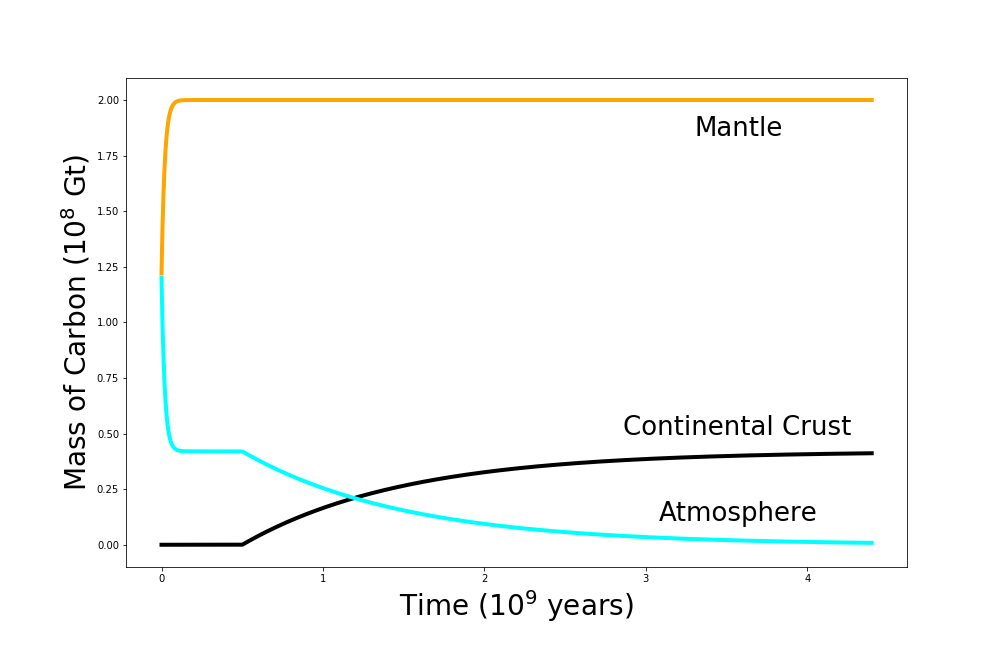
\includegraphics[scale=0.4]{Figures/ModelM-CC.png}
  \caption{Preliminary results of the time evolution of carbon cycle where the source of carbon in the continental crust is the mantle.}
  \label{Fig:ModelM-CC}
\end{figure}

If the influx of carbon due to subduction is equal to the outflux of carbon due to volcanism, then the mass of carbon in the mantle remains constant. Then, the source of carbon in the continental crust is the atmosphere. The same system of ODE is solved except that $\tau_{am} = 0$ and $^cJ_{cc-m} =\, ^cJ_{m-a}$. The time evolution of carbon in this alternative case is shown in Fig.~\ref{Fig:ModelA-CC}.

\begin{figure}[h!]
  \centering
  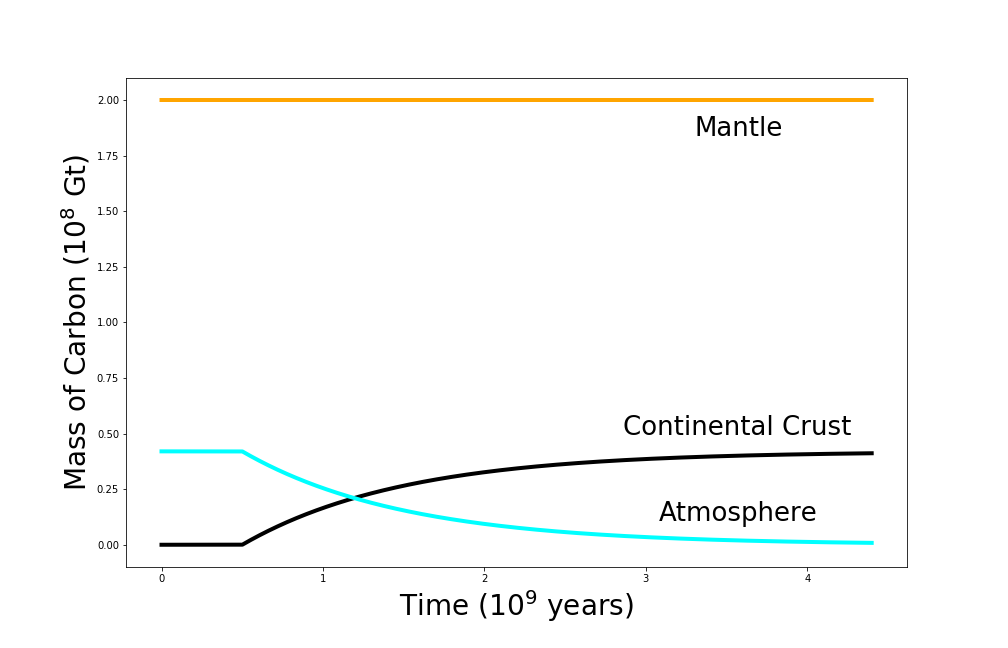
\includegraphics[scale=0.4]{Figures/ModelA-CC.png}
  \caption{Preliminary results of the time evolution of carbon cycle where the source of carbon in the continental crust is the atmosphere.}
  \label{Fig:ModelA-CC}
\end{figure}

A combination of the two limiting cases described above is also plausible. By introducing an independent parameter, we can then control what portion of the source of carbon in the continental crust is attributed to the atmosphere or mantle. A complete flow diagram of the proposed reservoir model is shown in Fig.~\ref{Fig:ReservoirFlowDiagram}

\begin{figure}[h!]
  \centering
  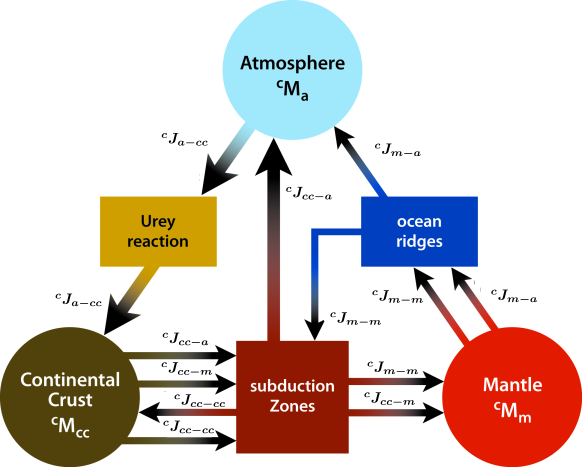
\includegraphics[scale=0.5]{Figures/RelabelJaniceFlowDiagram.png}
  \caption{A flow diagram showing the different reservoirs and pathways in our constructed box model.}
  \label{Fig:ReservoirFlowDiagram}
\end{figure}
